\begin{center}
  \textbf{Exercices Théoriques - Analyse Numérique - 2017 \\
  Section MA \\
  Prof. A. Quarteroni \\
  Séance 4 - Systèmes linéaires : méthodes directes et itératives}
\end{center}


\vspace{10mm}

\begin{ex}
Etudier l'existence et l'unicité de la factorisation $LU$ de Gauss des matrices suivantes :

\begin{equation*}
  A = \begin{bmatrix}
        1 & 2   \\
        1 & 2
      \end{bmatrix}
  , \quad
  B = \begin{bmatrix}
        0 & 1   \\
        1 & 0
      \end{bmatrix}
  , \quad
  C = \begin{bmatrix}
        0 & 1   \\
        0 & 2
      \end{bmatrix}
  .
\end{equation*}

Répéter l'exercice dans le cas où il est possible d'utiliser une matrice de pivots.
\end{ex}

\begin{sol}
On rappelle que si $M \in \R^{n \times n}$, la factorisation $LU$ de $M$ avec $l_{ii} = 1$ pour $i = 1, \dots , n$ existe et est unique si et seulement si les sous-matrices principales $M_{i}$ de $M$ d'ordre $i = 1, \dots , n - 1$ sont inversibles (voir Théorème 3.4 à la page 77 du livre).
Dans ce cas :

\begin{equation*}
  M = \begin{bmatrix}
        1       & 0   \\
        l_{21}  & 1
      \end{bmatrix}
      \begin{bmatrix}
        u_{11} & u_{12}   \\
        0      & u_{22}
      \end{bmatrix}
  =
      \begin{bmatrix}
        u_{11}          & u_{12}   \\
        l_{21} u_{11}   & l_{21} u_{12} + u_{22}
      \end{bmatrix}
  .
\end{equation*}

La matrice singulière $A$, dont la sous-matrice principale $A_{1} = 1$ est inversible, admet une unique factorisation $LU$.
La matrice inversible $B$ dont la sous-matrice $B_{1}$ est singulière n'admet pas de factorisation,
tandis que la matrice (singulière) $C$, dont la sous-matrice $C_{1}$ est singulière, admet une infinité de factorisations de la forme $C = L_{\beta} U_{\beta}$,
avec $l^{\beta}_{11} = 1$, $l^{\beta}_{21} = \beta$, $l^{\beta}_{22} = 1$, et $u^{\beta}_{11} = 0$, $u^{\beta}_{12} = 1$, $u^{\beta}_{22} = 2 - \beta, \ \quad \forall \beta \in \R$.

On se donne la possibilité d'utiliser une matrice de permutation pour les matrices $B$ et $C$ (la matrice $A$ n'en a pas besoin).
Pour $B$, si on utilise une matrice de permutation 

\begin{equation*}
  P = \begin{bmatrix}
        0 & 1   \\
        1 & 0
      \end{bmatrix}
      ,
\end{equation*}

on a que $PB = I$.
Par conséquent, la factorisation de $PB$ est triviale.

Pour $C$, il n'existe pas de matrice $P$ telle que le mineur principal d'ordre 1 de $PC$ est non nul.
En revanche, il existe une matrice

\begin{equation*}
  Q = \begin{bmatrix}
        0 & 1   \\
        1 & 0
      \end{bmatrix}
      ,
\end{equation*}

qui permute les colonnes telle que

\begin{equation*}
  CQ = \begin{bmatrix}
        1 & 0  \\
        2 & 0
      \end{bmatrix}
      .
\end{equation*}

Le mineur principal d'ordre 1 de $CQ$ est non nul, donc il existe une unique factorisation $LU$ de $CQ$.

\end{sol}

\begin{ex}
Soit $A$ la matrice donnée par

\begin{equation*}
  A = \begin{bmatrix}
        1  & 2  & 3  & 4  \\
        2  & 5  & 1  & 10  \\
        3  & 1  & 35 & 5  \\
        4  & 10 & 5  & 45 
      \end{bmatrix}
      ,
\end{equation*}

avec $\det \parent{A} > 0$.
Effectuer la factorisation de Cholesky de la matrice $A$, après avoir remarqué qu'une telle factorisation existe.

\end{ex}

\begin{sol}
La matrice est symétrique et définie positive.
En effet, la matrice est symétrique et tous les mineurs principaux dominants de $A$ sont positifs (critère de Sylvester).
On a vu au cours que les coefficients $h_{ij}$ de $H^{\top}$ (triangulaire inférieure), avec $A = H^{\top} H$, peuvent être calculés comme suit : $h_{11} = \sqrt{a_{11}}$ et, pour $i = 2, ... ,n$, on a

\begin{equation}
\label{eq:h}
  \begin{split}
      h_{ij}  = & \  \dfrac{1}{h_{jj}} \parent{a_{ij} - \sum_{k = 1}^{j-1} h_{ik} h_{jk}}, \quad j = 1, \dots, i-1; \\
      h_{ii}  = & \ \parent{a_{ii} - \sum_{k = 1}^{i-1} h_{ik}^{2}}^{1/2} .
  \end{split}
\end{equation}

On obtient ainsi

\begin{equation*}
  H^{\top} = \begin{bmatrix}
        1  & 0  & 0  & 0  \\
        2  & 1  & 0  & 0  \\
        3  & -5 & 1  & 0  \\
        4  & 2  & 3  & 4 
      \end{bmatrix}
      .
\end{equation*}

\end{sol}

\begin{ex}
\begin{enumerate}[label=\alph*)]
  \item En prenant $n = 1000$, écrire en \textsc{MATLAB} la matrice $n \times n$ suivante :
  
        \begin{equation*}
          A = \begin{bmatrix}
                1 & \textbf{1}^{\top}   \\
                \textbf{1} & -I_{n - 1}
              \end{bmatrix}
        \end{equation*}

        où $\textbf{1}$ est un vecteur colonne unitaire de longueur $n - 1$ et $I_{n-1}$ est la matrice identité $(n - 1) \times (n - 1)$.
        Ensuite calculer la factorisation $LU$ de la matrice $A$ avec \textsc{MATLAB} (en utilisant la commande \texttt{lu} avec $L$, $U$ et $P$ comme sorties ; écrire \texttt{help lu} pour apprendre comme utiliser la commande).

  \item Visualiser la structure des facteurs $L$ et $U$ et de la matrice de permutation $P$ (en utilisant la commande \texttt{spy}).
  
  \item Soient $\tilde{P}$ et $\tilde{Q}$ deux matrices de permutation.
        On considère maintenant la matrice $\tilde{A} = \tilde{P} A \tilde{Q}$ obtenue en effectuant une permutation des lignes avec $\tilde{P}$ et une permutation des colonnes avec $\tilde{Q}$ et on note par $\tilde{A} = \tilde{L} \tilde{U}$ la factorisation $LU$ de la matrice $\tilde{A}$.
        Trouver une permutation des lignes de $\tilde{P}$ et des colonnes de $\tilde{Q}$ telles que les facteurs $\tilde{L}$ et $\tilde{U}$ soient creux.

  \item Calculer une factorisation $\tilde{A} = \tilde{L} \tilde{U}$ de la matrice $\tilde{A}$ à l'aide de la commande \texttt{lu} et visualiser la structure des facteurs $\tilde{L}$ et $\tilde{U}$.
  
  \item Transformer au format creux (en utilisant la commande \texttt{sparse}) les matrices $L$, $U$ du point (a), et les matrices $\tilde{L}$, $\tilde{U}$ du point (d).
        En utilisant la commande \texttt{whos} comparer la taille en mémoire de ces matrices.
        Que peut-on remarquer ?
\end{enumerate}
\end{ex}

\begin{sol}
\begin{enumerate}[label=\alph*)]
  \item Pour construire la matrice
  
        \begin{equation*}
          A = \begin{bmatrix}
                1 & \textbf{1}^{\top}   \\
                \textbf{1} & -I_{n - 1}
              \end{bmatrix}
        \end{equation*}
        
        on utilise en \textsc{MATLAB} les commandes suivantes
        
\begin{verbatim}
n = 1000;
a11 = 1;
a12 = ones(1, n-1);
a21 = ones(n-1, 1);
a22 = -eye(n-1,n-1);
A = [a11,a12;a21,a22];
\end{verbatim}

      Ensuite, pour calculer la factorisation $LU$, on utilise la commande :
      
\begin{verbatim}
[L,U,P] = lu(A);
\end{verbatim}

  \item Pour visualiser la structure des facteurs $L$ et $U$, on écrit
  
\begin{verbatim}
figure(1)
spy(L)
figure(2)
spy(U)
\end{verbatim}  

    On voit sur la Figure \ref{fig:lu} que les facteurs sont pleins :

    \begin{figure}[h!]
      \begin{subfigure}[b]{0.5\linewidth}
        \centering
        \includegraphics[scale=0.4]{s4/matlab/L-eps-converted-to.pdf} 
        %\caption{Interpolation of $f$ using NCS \\ with $8+2$ points} 
        %\label{fig:q11_n8} 
      \end{subfigure}
      \begin{subfigure}[b]{0.5\linewidth}
        \centering
        \includegraphics[scale=0.4]{s4/matlab/U-eps-converted-to.pdf} 
        %\caption{Interpolation of $f$ using NCS \\ with $8+2$ points} 
        %\label{fig:q11_n8} 
      \end{subfigure} 
      \caption{Structure des matrices $L$ (à gauche) et $U$ (à droite) telles que $A = LU$.}
      \label{fig:lu}
    \end{figure}   
    
  \item On peut permuter la première ligne de $A$ avec la dernière, ainsi que la première colonne de $A$ avec la dernière, en utilisant la matrice de permutation $P$ donnée par
  
  
  \begin{equation*}
    P = \begin{bmatrix}
      0       & 0       & \dots   & 0       & 1 \\
      0       & 1       & \dots   & 0       & 0 \\
      \vdots  & \vdots  & \ddots  & \vdots  & \vdots \\
      0       & 0       & \dots   & 1       & 0 \\
      1       & 0       & \dots   & 0       & 0
        \end{bmatrix}
        ,
  \end{equation*}
  
  et en exécutant le produit $\tilde{A} = PAP$ : 
  
\begin{verbatim}
P = zeros(n,n);
P(1, n) = 1;
P(n, 1) = 1;
P(2:n-1, 2:n-1) = eye(n-2,n-2);
tildeA = P*A*P;
\end{verbatim} 

  \item La factorisation $LU$ de $\tilde{A}$, telle que $\tilde{A} = \tilde{L} \tilde{U}$ , ainsi que les structures des matrices $\tilde{L}$ et $\tilde{U}$, sont données par :
  
\begin{verbatim}
[tildeL, tildeU] = lu(tildeA);
figure(3)
spy(tildeL)
figure(4)
spy(tildeU)
\end{verbatim} 
    
   On trouve les structures pésentées dans la Figure \ref{fig:tildelu}.
   
   \begin{figure}[h!]
     \begin{subfigure}[b]{0.5\linewidth}
       \centering
       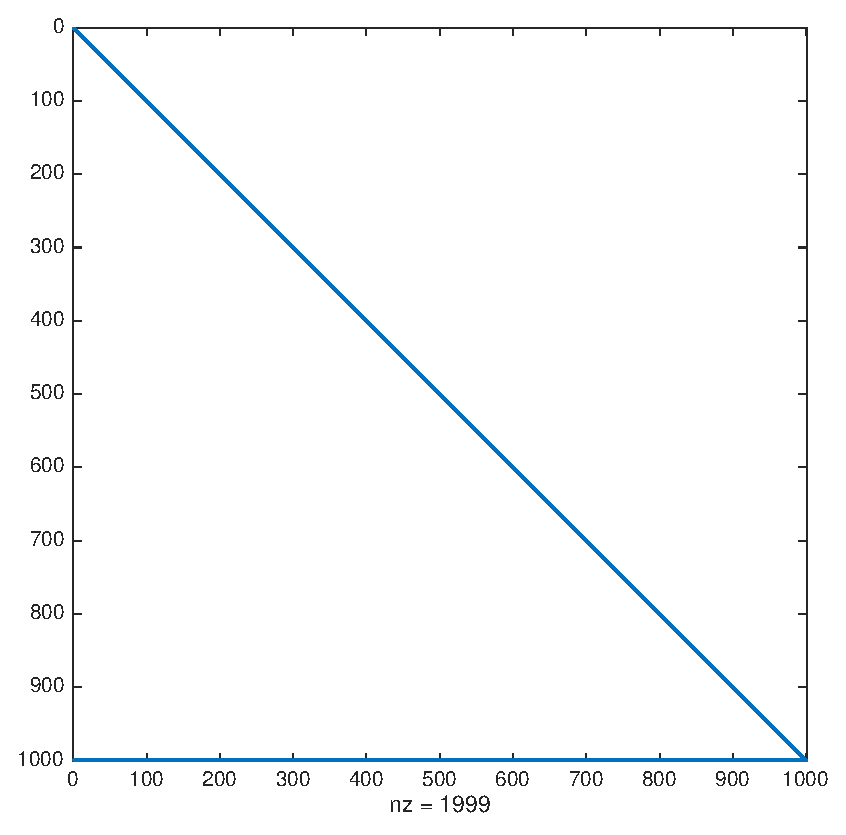
\includegraphics[scale=0.4]{s4/matlab/tildeL} 
       %\caption{Interpolation of $f$ using NCS \\ with $8+2$ points} 
       %\label{fig:q11_n8} 
     \end{subfigure}
     \begin{subfigure}[b]{0.5\linewidth}
       \centering
       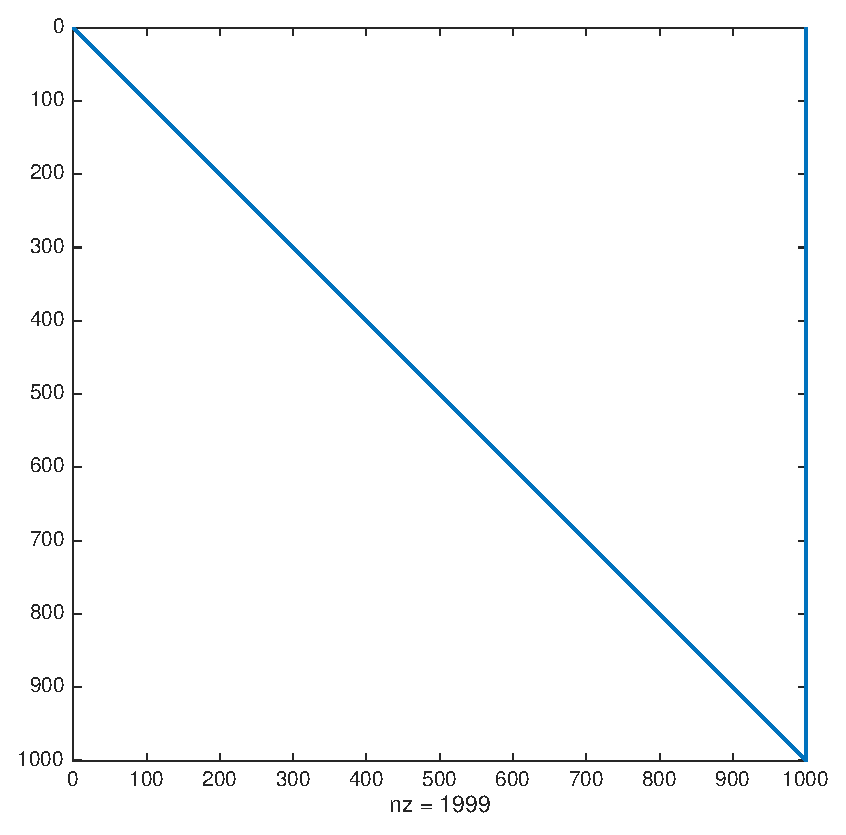
\includegraphics[scale=0.4]{s4/matlab/tildeU} 
       %\caption{Interpolation of $f$ using NCS \\ with $8+2$ points} 
       %\label{fig:q11_n8} 
     \end{subfigure} 
     \caption{Structure des matrices $\tilde{L}$ (à gauche) et $\tilde{U}$ (à droite) telles que $\tilde{A} = \tilde{L} \tilde{U}$.}
     \label{fig:tildelu}
   \end{figure}  
   
   
   
   \item On peut noter que le nombre d'éléments non nuls passe de 500500 à 1999, donc il est 250 fois plus petit !
         Cette différence devient importante surtout quand on utilise un format de représentation des matrices creuses qui ne garde que les entrées non-nulles.
         Cela est fait en \textsc{MATLAB} à l'aide de la commande \texttt{sparse}.
         Normalement, si on travaille avec des matrices creuses et qu'on les converties au format creux, on gagne en memoire et en performance.
         Pour cet exemple, on peut voir la différence en tapant
         
\begin{verbatim}
sparseU = sparse(U);
sparseL = sparse(L);
sparse_tildeU = sparse(tildeU);
sparse_tildeL = sparse(tildeL);
whos
\end{verbatim} 

On trouve

\lstinputlisting{s4/matlab/out3.txt}


On voit que l'utilisation de la mémoire pour des matrices pleines est de 8 MB (en fait, comme les entrées sont des \texttt{double}, donc 8 Bytes, 8 * 1.000 * 1.000 = 8.000.000 Bytes = 8 MB).
Pour la première factorisation ($LU$), l'utilisation est même plus grande avec le format \texttt{sparse}, tandis que si on utilise la deuxième factorisation ($\tilde{L} \tilde{U}$), chaque facteur occupe moins de 40 KB, c'est-à-dire plus de 200 fois moins que dans le premier cas.


         
  
  Les figures de cet exercice sont obtenues avec le script \texttt{ex3.m}.

  \lstinputlisting{s4/matlab/ex3.m}





\end{enumerate}
\end{sol}

\begin{ex}
En considérant la matrice de Hilbert $A \in \R^{n \times n}$

\begin{equation*}
  A = \begin{bmatrix}
        1                & 1/2      & 1/3      & 1/4      & \dots \\
        1/2      & 1/3      & 1/4      & \dots            &       \\
        1/3      & \vdots           &                  &                  &       \\
        \vdots           &                  &                  &                  &      
      \end{bmatrix}
      \quad \quad 
      A_{ij} = \dfrac{1}{i+j-1}
      ;
\end{equation*}

\begin{enumerate}[label=\alph*)]
  \item Calculer avec \textsc{MATLAB} les éléments de la matrice $A$ avec $n = 10$ (en utilisant la commande \texttt{hilb}) et le nombre de conditionnement $K_{2}\parent{A}$ avec la commande \texttt{cond}.
        Enregistrer les nombres de conditionnement calculés pour $n = 1, \dots , 10$ dans un vecteur avec 10 composantes.
        
  \item Visualiser sur un graphe en échelle semilogarithmique (linéaire sur les abscisses et logarithmique sur les ordonnées) la valeur de $K_{2}\parent{A}$ en fonction de $n$, pour $1 \leq n \leq 10$ en utilisant la commande \texttt{semilogy}.
        En déduire que $K_{2}\parent{A}$ se comporte comme $e^{\alpha n}$.
        
  \item Construire un vecteur colonne $\BoldX_{e x}$ aléatoire avec $n$ composantes en utilisant la commande \texttt{rand} et calculer le vecteur $\BoldB = A \BoldX_{e x}$.
        Pour chaque $n = 1, 2, \dots , 10$ résoudre le système linéaire $A \BoldX = \BoldB$ avec la commande \textbackslash \ qui met en oeuvre une méthode directe, et calculer l'erreur relative
  
        \begin{equation}
        \label{eq:err}
          \varepsilon^{r} = \dfrac{\norm{\BoldX - \BoldX_{e x}}}{\norm{\BoldX_{e x}}}.
        \end{equation}
        
        Visualiser l'erreur sur un graphe en échelle semilogarithmique et en déduire que cette erreur se conduit comme $K_{2}\parent{A}$.
        Visualiser ensemble l'erreur relative $\varepsilon^{r}$ et son estimation $\tilde{\varepsilon}^{r}$ en échelle semilogarithmique, où $\BoldR$ est le résidu et $\tilde{\varepsilon}^{r}$ est défini comme
        
        \begin{equation}
        \label{eq:tildeerr}
          \tilde{\varepsilon}^{r}
          = K_{2}\parent{A} \frac{\norm{\BoldR}}{\norm{\BoldB}}.
        \end{equation}
        
         
        
\end{enumerate}



\end{ex}

\begin{sol}
\begin{enumerate}[label=\alph*)]
  \item D'abord on apprend que
  
\begin{verbatim}
help hilb
 HILB   Hilbert matrix.
      HILB(N) is the N by N matrix with elements 1/(i+j-1),
      which is a famous example of a badly conditioned matrix.
\end{verbatim}
  
  On peut calculer les quantités nécessaires avec les commandes suivantes, dans une boucle \texttt{for} pour $n = 1, 2, \dots, 10$: 
  
\begin{verbatim}
for n=1:10
    A = hilb(n);
    KA(n) = cond(A);
end 
\end{verbatim}

  \item Le conditionnement de la matrice $A$ est enregistré dans le vecteur \texttt{KA}, qui vaut
  
        \lstinputlisting{s4/matlab/KA.txt}
  
        et son comportement en fonction de $n$ peut être visualisé avec les commandes suivantes :

\begin{verbatim}
figure(1);
semilogy([1:1:10],KA,'r');
grid;
xlabel('n');
ylabel('K(A)');
\end{verbatim}

      On peut observer à la Figure \ref{fig:KA} que le conditionnement a une comportement linéaire sur le graphique, c'est-à-dire $K_{2}\parent{A}$ croit (presque) exponentiellement en fonction de $n$.
      
      \begin{figure}[h!]
        \centering
        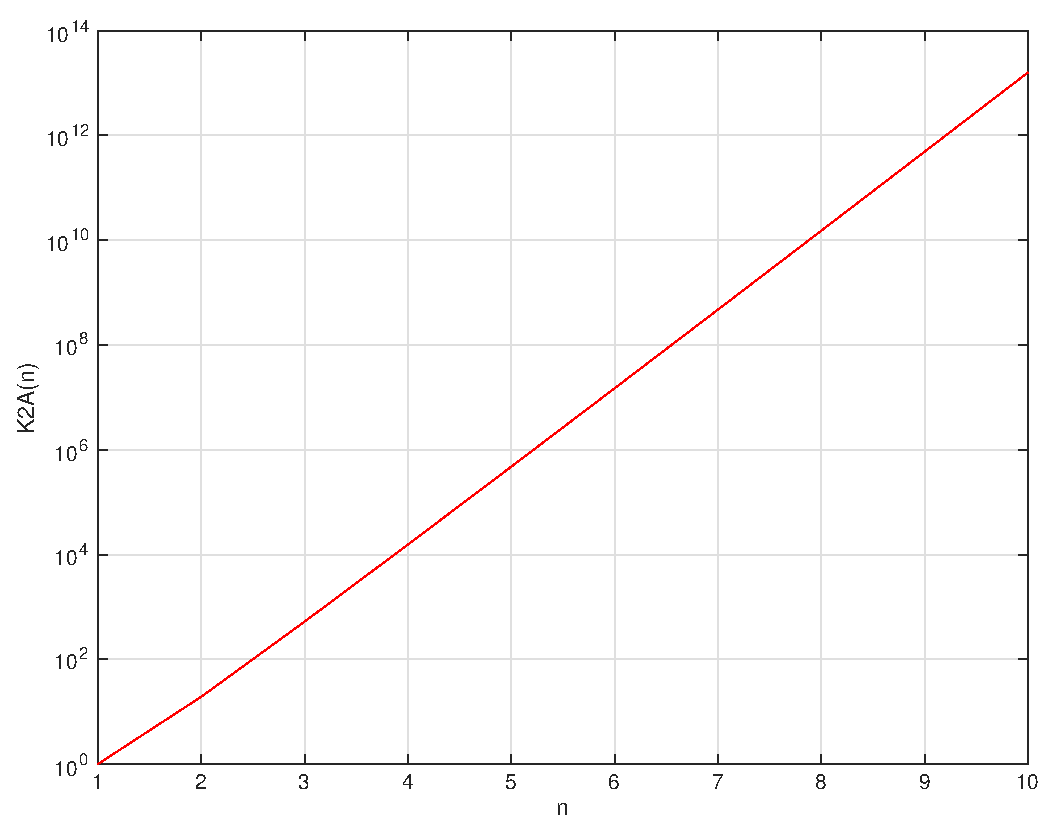
\includegraphics[scale = 0.5]{s4/matlab/KA.eps}
        \caption{Graphique du conditionnement de la matrice de Hilbert en fonction de $n$ ; l'échelle est linéaire sur les abscisses et logarithmique sur les ordonnées.}
        \label{fig:KA}
      \end{figure}

      \item On veut construire un vecteur colonne $\BoldX_{e x}$ aléatoire avec $n$ composantes, calculer le vecteur $\BoldB = A \BoldX_{e x}$, résoudre (pour chaque $n = 1, 2, \dots , 10$) le système linéaire $A \BoldX = \BoldB$ et calculer l'erreur relative

      \begin{equation*}
        \varepsilon^{r} = \dfrac{\norm{\BoldX - \BoldX_{e x}}}{\norm{\BoldX_{e x}}};
      \end{equation*}
      
      on peut utiliser le code suivant :
      
\begin{verbatim}
for n=1:10
    A = hilb(n);
    KA(n) = cond(A);
    xex = rand(n,1);
    b = A * xex;
    x = A\b;
    err(n) = norm(x-xex)/norm(xex);
end
\end{verbatim}

    Ensuite, pour visualiser le comportement du conditionnement et de l'erreur relative $\varepsilon^{r}$ sur le même graphique, on peut taper :
    
\begin{verbatim}
figure(2);
semilogy([1:1:10], KA, 'r', [1:1:10], err, 'h');
grid;
xlabel('n');
ylabel('KA(n) & err(n)');
\end{verbatim}

\begin{figure}[h!]
  \begin{subfigure}[b]{0.5 \linewidth}
    \centering
    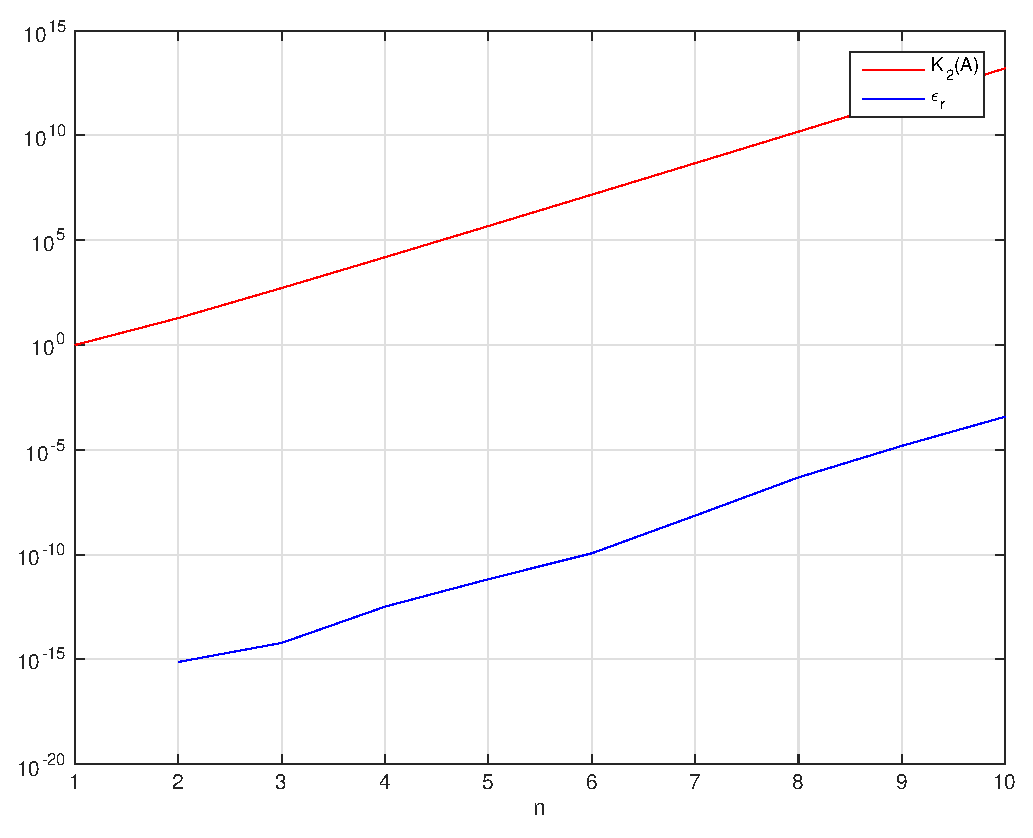
\includegraphics[scale=0.4]{s4/matlab/KVSErr} 
    \caption{$K$ et $\varepsilon^{r}$ en fonction de $n$.} 
    \label{figKAAndErra} 
  \end{subfigure}
  \begin{subfigure}[b]{0.5 \linewidth}
    \centering
    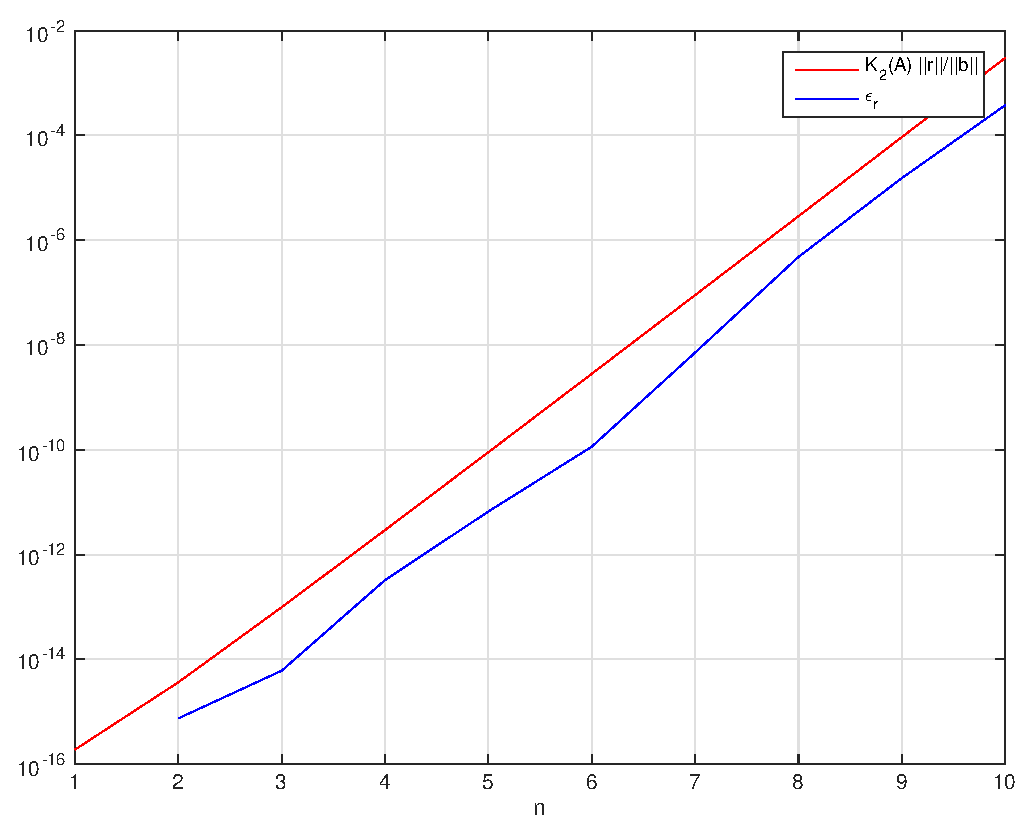
\includegraphics[scale=0.4]{s4/matlab/ErrVSTildeErr} 
    \caption{$\tilde{\varepsilon}^{r}$ et $\varepsilon^{r}$ en function de $n$.} 
    \label{figKAAndErrb} 
  \end{subfigure} 
  \caption{A gauche, Figure 4(a) : Graphique du conditionnement de la matrice de Hilbert, $K$, et de l'erreur relative, $\varepsilon^{r}$, définie à l'équation \eqref{eq:err}, en fonction de $n$. \\
  A droite, Figure 4(b) : Graphique de l'estimation de l'erreur relative, $\tilde{\varepsilon}^{r}$, définie à l'équation \eqref{eq:tildeerr}, et de l'erreur relative, $\varepsilon^{r}$, en function de $n$. \\
  L'échelle est linéaire sur les abscisses et logarithmique sur les ordonnées.}
  \label{figKAAndErr}
\end{figure} 


Le graphique à la Figure \ref{figKAAndErr} montre le conditionnement (ligne rouge) et l'erreur (ligne bleu) en fonction de $n$ dans une échelle semi-logarithmique.
On peut observer que l'erreur relative se comporte de la même façon que le conditionnement, même si elle est plus petite.
Cela confirme le fait que, plus le conditionnement de la matrice est grand, plus les erreurs d'arrondi sont amplifiées dans la résolution du système linéaire, conduisant à une erreur relative toujours plus grande, en accord avec l'inégalité suivante :

\begin{equation*}
  \dfrac{\norm{\delta \BoldX}}{\norm{\BoldX}}
  \leq \dfrac{K\parent{A}}{1 - K\parent{A} \norm{\delta A} / \norm{A}}
  \parent{\dfrac{\norm{\delta \BoldB}}{\norm{\BoldB}} + \dfrac{\norm{\delta A}}{\norm{A}}}
  .
\end{equation*}

Les figures de cet exercice sont obtenues avec le script \texttt{ex4.m}.

\lstinputlisting{s4/matlab/ex4.m}
    
      

\end{enumerate}




\end{sol}